% ------------------------------------------------------------------------
% LNCS LaTeX Paper ******************************************************
% ------------------------------------------------------------------------
% Submitted:      July 12 2005
% Final Version:  
% Accepted:       
% ------------------------------------------------------------------------
% This is a journal top-matter template file for use with AMS-LaTeX.
%%%%%%%%%%%%%%%%%%%%%%%%%%%%%%%%%%%%%%%%%%%%%%%%%%%%%%%%%%%%%%%%%%%%%%%%%%

%\documentclass{tran-l}
%\documentclass[twocolumn]{amsart}
%\documentclass[]{amsart}
\documentclass[]{llncs}
\usepackage[all,knot]{xy}

\newif\ifpdf
\ifx\pdfoutput\undefined
\pdffalse % we are not running PDFLaTeX
\else
\pdfoutput=1 % we are running PDFLaTeX
\pdftrue
\fi

\ifpdf
\usepackage[pdftex]{graphicx}
\else
\usepackage{graphicx}
\fi
%\usepackage[pdftex]{graphicx}

%\documentclass[]{entcs}
%\usepackage[]{prentcsmacro}

%\usepackage[active]{srcltx} % SRC Specials for DVI Searching
\usepackage {mathpartir}
%\usepackage {listings}
%\usepackage {array}
\usepackage{url}

% From Allen's stable.
%\usepackage{bigpage}
\usepackage{bcprules}
\usepackage{code}
\usepackage{amsfonts}
\usepackage{amstext}
\usepackage{latexsym}
\usepackage{amssymb}
%\usepackage{caption}
\usepackage{multicol}


% Double brackets
\newcommand{\ldb}{[\![}
\newcommand{\rdb}{]\!]}
\newcommand{\ldrb}{(\!(}
\newcommand{\rdrb}{)\!)}
\newcommand{\lliftb}{\langle\!|}
\newcommand{\rliftb}{|\!\rangle}
% \newcommand{\lpquote}{\langle}
% \newcommand{\rpquote}{\rangle}
% \newcommand{\lpquote}{\lceil}
% \newcommand{\rpquote}{\rceil}
\newcommand{\lpquote}{\ulcorner}
\newcommand{\rpquote}{\urcorner}
\newcommand{\newkw}{\nu}

% SYNTAX
\newcommand{\id}[1]{\texttt{#1}}
\newcommand{\none}{\emptyset}
\newcommand{\eps}{\epsilon}
\newcommand{\set}[1]{\{#1\}}
\newcommand{\rep}[2]{\id{\{$#1$,$#2$\}}}
\newcommand{\elt}[2]{\id{$#1$[$#2$]}}
\newcommand{\infinity}{$\infty$}

\newcommand{\pzero}{\mathbin{0}}
\newcommand{\seq}{\mathbin{\id{,}}}
\newcommand{\all}{\mathbin{\id{\&}}}
\newcommand{\choice}{\mathbin{\id{|}}}
\newcommand{\altern}{\mathbin{\id{+}}}
\newcommand{\juxtap}{\mathbin{\id{|}}}
\newcommand{\concat}{\mathbin{.}}
\newcommand{\punify}{\mathbin{\id{:=:}}}
\newcommand{\fuse}{\mathbin{\id{=}}}
\newcommand{\scong}{\mathbin{\equiv}}
\newcommand{\nameeq}{\mathbin{\equiv_N}}
\newcommand{\alphaeq}{\mathbin{\equiv_{\alpha}}}
\newcommand{\names}[1]{\mathbin{\mathcal{N}(#1)}}
\newcommand{\freenames}[1]{\mathbin{\mathcal{FN}(#1)}}
\newcommand{\boundnames}[1]{\mathbin{\mathcal{BN}(#1)}}
%\newcommand{\lift}[2]{\texttt{lift} \; #1 \concat #2}
\newcommand{\binpar}[2]{#1 \juxtap #2}
\newcommand{\outputp}[2]{#1 \id{[} #2 \id{]}}
\newcommand{\prefix}[3]{#1 \id{(} #2 \id{)} \concat #3}
\newcommand{\lift}[2]{#1 \lliftb #2 \rliftb}
\newcommand{\quotep}[1]{\lpquote #1 \rpquote}
\newcommand{\dropn}[1]{\rpquote #1 \lpquote}

\newcommand{\newp}[2]{\id{(}\newkw \; #1 \id{)} #2}
\newcommand{\bangp}[1]{\id{!} #1}

\newcommand{\substp}[2]{\id{\{} \quotep{#1} / \quotep{#2} \id{\}}}
\newcommand{\substn}[2]{\id{\{} #1 / #2 \id{\}}}

\newcommand{\psubstp}[2]{\widehat{\substp{#1}{#2}}}
\newcommand{\psubstn}[2]{\widehat{\substn{#1}{#2}}}

\newcommand{\applyp}[2]{#1 \langle #2 \rangle}
\newcommand{\absp}[2]{\id{(} #1 \id{)} #2}

\newcommand{\transitions}[3]{\mathbin{#1 \stackrel{#2}{\longrightarrow} #3}}
\newcommand{\meaningof}[1]{\ldb #1 \rdb}
\newcommand{\pmeaningof}[1]{\ldb #1 \rdb}
\newcommand{\nmeaningof}[1]{\ldrb #1 \rdrb}

\newcommand{\Proc}{\mathbin{Proc}}
\newcommand{\QProc}{\quotep{\mathbin{Proc}}}

\newcommand{\entailm}{\mathbin{\vdash_{\mathfrak m}}} %matching
\newcommand{\entailp}{\mathbin{\vdash_{\mathfrak p}}} %behavioral
\newcommand{\entailv}{\mathbin{\vdash_{\mathfrak v}}} %validation
\newcommand{\congd}{\mathbin{\equiv_{\mathfrak d}}}
\newcommand{\congs}{\mathbin{\equiv_{\mathfrak s}}}
\newcommand{\congp}{\mathbin{\equiv_{\mathfrak p}}}
%\newcommand{\logequiv}{\mathbin{\leftrightarrow}}

\newcommand{\barb}[2]{\mathbin{#1 \downarrow_{#2}}}
\newcommand{\dbarb}[2]{\mathbin{#1 \Downarrow_{#2}}}

% From pi-duce paper
\newcommand{\red}{\rightarrow}
\newcommand{\wred}{\Rightarrow}
\newcommand{\redhat}{\hat{\longrightarrow}}
\newcommand{\lred}[1]{\stackrel{#1}{\longrightarrow}} %transitions
\newcommand{\wlred}[1]{\stackrel{#1}{\Longrightarrow}}

\newcommand{\opm}[2]{\overline{#1} [ #2 ]} % monadic
\newcommand{\ipm}[2]{{#1} ( #2 )} 
\newcommand{\ipmv}[2]{{#1} ( #2 )} % monadic
\newcommand{\parop}{\;|\;}		% parallel operator
\newcommand{\patmatch}[3]{#2 \in #3 \Rightarrow #1}
\newcommand{\sdot}{\, . \,}		% Space around '.'
\newcommand{\bang}{!\,}
%\newcommand{\fuse}[1]{\langle #1 \rangle}		
\newcommand{\fusion}[2]{#1 = #2} % fusion prefix/action
\newcommand{\rec}[2]{\mbox{\textsf{rec}} \, #1. \, #2}
\newcommand{\match}[2]{\mbox{\textsf{match}} \; #1 \; \mbox{\textsf{with}} \; #2}
\newcommand{\sep}{:}
\newcommand{\val}[2]{\mbox{\textsf{val}} \; #1 \; \mbox{\textsf{as}} \; #2}

\newcommand{\rel}[1]{\;{\mathcal #1}\;} %relation
\newcommand{\bisim}{\stackrel{.}{\sim}_b} %bisimilar
\newcommand{\wb}{\approx_b} %weak bisimilar
\newcommand{\bbisim}{\stackrel{\centerdot}{\sim}} %barbed bisimilar
\newcommand{\wbbisim}{\stackrel{\centerdot}{\approx}} %weak barbed bisimilar
\newcommand{\bxless}{\lesssim}	%expansion less (amssymb required)
\newcommand{\bxgtr}{\gtrsim}	%expansion greater (amssymb required)
\newcommand{\beq}{\sim}		%barbed congruent
\newcommand{\fwbeq}{\stackrel{\circ}{\approx}}	%weak barbed congruent
\newcommand{\wbeq}{\approx}	%weak barbed congruent
\newcommand{\sheq}{\simeq}	%symbolic hypereq
\newcommand{\wbc}{\approx_{cb}}

% rho logic

\newcommand{\ptrue}{\mathbin{true}}
\newcommand{\psatisfies}[2]{#1 \models #2}
\newcommand{\pdropf}[1]{\rpquote #1 \lpquote}
\newcommand{\plift}[2]{#1 \lliftb #2 \rliftb}
\newcommand{\pprefix}[3]{\langle #1 ? #2 \rangle #3}
\newcommand{\pgfp}[2]{\textsf{rec} \; #1 \mathbin{.} #2}
\newcommand{\pquant}[3]{\forall #1 \mathbin{:} #2 \mathbin{.} #3}
\newcommand{\pquantuntyped}[2]{\forall #1 \mathbin{.} #2}
\newcommand{\riff}{\Leftrightarrow}

\newcommand{\PFormula}{\mathbin{PForm}}
\newcommand{\QFormula}{\mathbin{QForm}}
\newcommand{\PropVar}{\mathbin{\mathcal{V}}}

% End piduce contribution

\newcommand{\typedby}{\mathbin{\:\colon}}
\newcommand{\mixedgroup}[1]{\id{mixed($#1$)}}
\newcommand{\cast}[2]{\id{CAST AS} \; #1 \; (#2)}
\newcommand{\bslsh}{\mathbin{\id{\\}}}
\newcommand{\bslshslsh}{\mathbin{\id{\\\\}}}
\newcommand{\fslsh}{\mathbin{\id{/}}}
\newcommand{\fslshslsh}{\mathbin{\id{//}}}
\newcommand{\bb}[1]{\mbox{#1}}
\newcommand{\bc}{\mathbin{\mathbf{::=}}}
\newcommand{\bm}{\mathbin{\mathbf\mid}}
\newcommand{\be}{\mathbin{=}}
\newcommand{\bd}{\mathbin{\buildrel {\rm \scriptscriptstyle def} \over \be}}
\newcommand{\category}[1]{\mbox{\bf #1}}

%GRAMMAR
\newlength{\ltext}
\newlength{\lmath}
\newlength{\cmath}
\newlength{\rmath}
\newlength{\rtext}

\settowidth{\ltext}{complex type name}
\settowidth{\lmath}{$xxx$}
\settowidth{\cmath}{$::=$}
\settowidth{\rmath}{\id{attributeGroup}}
\settowidth{\rtext}{repetition of $g$ between $m$ and $n$ times}

\newenvironment{grammar}{
  \[
  \begin{array}{l@{\quad}rcl@{\quad}l}
  \hspace{\ltext} & \hspace{\lmath} & \hspace{\cmath} & \hspace{\rmath} & \hspace{\rtext} \\
}{
  \end{array}\]
}

% Over-full v-boxes on even pages are due to the \v{c} in author's name
%\vfuzz2pt % Don't report over-full v-boxes if over-edge is small

% THEOREM Environments ---------------------------------------------------
% MATH -------------------------------------------------------------------
 \newcommand{\veps}{\varepsilon}
 \newcommand{\To}{\longrightarrow}
 \newcommand{\h}{\mathcal{H}}
 \newcommand{\s}{\mathcal{S}}
 \newcommand{\A}{\mathcal{A}}
 \newcommand{\J}{\mathcal{J}}
 \newcommand{\M}{\mathcal{M}}
 \newcommand{\W}{\mathcal{W}}
 \newcommand{\X}{\mathcal{X}}
 \newcommand{\BOP}{\mathbf{B}}
 \newcommand{\BH}{\mathbf{B}(\mathcal{H})}
 \newcommand{\KH}{\mathcal{K}(\mathcal{H})}
 \newcommand{\Real}{\mathbb{R}}
 \newcommand{\Complex}{\mathbb{C}}
 \newcommand{\Field}{\mathbb{F}}
 \newcommand{\RPlus}{\Real^{+}}
 \newcommand{\Polar}{\mathcal{P}_{\s}}
 \newcommand{\Poly}{\mathcal{P}(E)}
 \newcommand{\EssD}{\mathcal{D}}
 \newcommand{\Lom}{\mathcal{L}}
 \newcommand{\States}{\mathcal{T}}
 \newcommand{\abs}[1]{\left\vert#1\right\vert}
% \newcommand{\set}[1]{\left\{#1\right\}}
%\newcommand{\seq}[1]{\left<#1\right>}
 \newcommand{\norm}[1]{\left\Vert#1\right\Vert}
 \newcommand{\essnorm}[1]{\norm{#1}_{\ess}}

%%% NAMES
\newcommand{\Names}{{\mathcal N}}
\newcommand{\Channels}{{\sf X}}
\newcommand{\Variables}{{\mathcal V}}
\newcommand{\Enames}{{\mathcal E}}
\newcommand{\Nonterminals}{{\mathcal S}}
\newcommand{\Pnames}{{\mathcal P}}
\newcommand{\Dnames}{{\mathcal D}}
\newcommand{\Types}{{\mathcal T}}

\newcommand{\fcalc}{fusion calculus}
\newcommand{\xcalc}{${\mathfrak x}$-calculus}
\newcommand{\lcalc}{$\lambda$-calculus}
\newcommand{\pic}{$\pi$-calculus}
\newcommand{\spic}{spi-calculus}
\newcommand{\rhoc}{$\rho$-calculus}
\newcommand{\rhol}{$\rho$-logic}
\newcommand{\hcalc}{highwire calculus}
\newcommand{\dcalc}{data calculus}
%XML should be all caps, not small caps. --cb
%\newcommand{\xml}{\textsc{xml}}
\newcommand{\xml}{XML} 


\newcommand{\papertitle}{Knots as processes: a new kind of invariant}
% use static date to preserve date of actual publication
\newcommand{\paperversion}{Draft Version 0.1 - December 19, 2004}

\newenvironment{toc}
{
\begin{list}{}{
   \setlength{\leftmargin}{0.4in}
   \setlength{\rightmargin}{0.6in}
   \setlength{\parskip}{0pt}
 } \item }
{\end{list}}

\newenvironment{narrow}
{
\begin{list}{}{
   \setlength{\leftmargin}{0.4in}
   \setlength{\rightmargin}{0.6in}
 } \item }
{\end{list}}

\def\lastname{Meredith and Snyder}
%%% ----------------------------------------------------------------------

\begin{document}

%\begin{frontmatter}
\title{Knots as processes: a new kind of invariant}
\titlerunning{Namespace logic}

\author{ L.G. Meredith\inst{1} \and David F. Snyder\inst{2} }
\institute{ CXO, Biosimilarity\\ 505 N72nd St, Seattle, WA 98103, USA, \\
  \email{ lgreg.meredith@gmail.com } \\
  \and Associate Professor of Mathematics\\ Dept of Mathematics\\ Texas State University\\ 601 University Drive \\ San Marcos, TX 78666 \\
  \email{ dsnyder@txstate.edu }
} 

\maketitle              % typeset the title of the contribution

%%% ----------------------------------------------------------------------

\begin{abstract}

          We exhibit an encoding of knots into processes in the
          $\pi$-calculus such that knots are ambient isotopic if and
          only their encodings are weakly bisimilar.

\end{abstract}

% \begin{keyword}
% concurrency, message-passing, process calculus, reflection, program logic
% \end{keyword}

%\end{frontmatter}

\section{Introduction and motivation}

Recent research in concurrency theory has led many to consider
geometric interpretations of concurrent computation such as Goubault's
investigations of higher-order automata
\cite{DBLP:conf/concur/GoubaultJ92}
\cite{DBLP:journals/mscs/Goubault00a} and Herlihy's application of
homology theory \cite{DBLP:journals/entcs/HerlihyRT02}. In this paper,
however, we switch the roles of the domain of investigation and the
tool by which to investigate it, and find ourselves returning to a
more traditional mathematical activity of assocating an algebraic
invariant to a spatial entity -- with a twist. \footnote{Pun
  gratefully accepted ;-).} More specifically, we investigate the use
of the algebras of concurrency theory to derive invariants for knots,
exhibiting an encoding of knots as processes in the $\pi$-calculus.

The encoding has the nice property that two knots are ambient isotopic
if and only if their encodings as processes are weakly
bisimilar. While this makes clear that the invariant is particularly
discriminating, we see another motivation for investigating knots from
this perspective. Specifically, bisimulation has proven to be an
incredibly powerful and flexible proof principle, adaptable to a wide
range of situations and admitting a number of potent up-to techniques
\cite{DBLP:conf/lics/Sangiorgi04}
\cite{DBLP:conf/mfcs/Sangiorgi95}. Thus, while Goubault and others
have sought insight into the equivalence of computational behavior by
looking at the equivalence of spaces, we think the dialogue is really
two-way. In particular, what we have learned from the past several
decades of investigation into notions of the equivalence of
computational behavior may bear fruit in the study of the equivalence
of spaces.

\subsection{Overview and summary of contributions}

In section \ref{Pinut} we give a brief review of the polyadic $\pi$-calculus,
immediately following that with a review of the primary results from
knot theory needed to state and prove our main theorem. Next, we
introduce the intuitions behind the encoding, sketching the general
shape and walking through the procedure in the case of the trefoil. We
follow this with the details of the encoding. This puts us in a
position to state and prove the main theorem, which we do in section
\ref{MainThm}. In the penultimate section we discussion some of the results
following from this method of encoding, illustrating a way to
interpret knot composition as parallel composition and a way to
interpret the Kauffman bracket (and hence a number of other knot
invariants) in this setting. Finally, we state some conclusions and
adumbrate some directions for future research.

\section{The $\pi$-calculus in a nutshell} \label{Pinut}

Since Milner's seminal paper \textit{Functions as processes}
\cite{FunctionsAsProcesses} \footnote{From which this paper takes
  inspiration for half its title...}, it has become standard to
present process calculi in a manner strongly reminiscent of the
presentation of an algebra via generators and relations. The grammar
generating the set of processes may be seen as a generalization of
generators and the structural equivalence may be seen as the relations
over the freely generated set. 

In this sense, the process calculi fit well into the standard zoo of
algebraic structures, resembling vector spaces in the sense that they
are built out of two kinds of fundamental building blocks --
i.e. vector spaces are built out of scalars and vectors while
process calculi are built out of names and processes. What
distinguishes them from these more traditional algebraic structures is
the introduction of an additional relation, called reduction, that is
neither a priori reflexive or symmetric, representing the evolution or
dynamics of a process. Thus, these structures have an explicit
representation of computation, unlike structures such as vector spaces
where dynamics is introduced via functions between such structures.

It is noteworthy that several other `computational calculi' also admit
similar algebraic presentations. The lambda calculi, as a family,
provide a canonical example: term grammar as generalized generators;
alpha-equivalence as relations; and beta-reduction as the explicit
account of dynamics. We submit that such computational calculi may
quite generally constitute an interesting class to mine for
topological invariants -- especially in light of bisimulation
techniques.

\subsection{\pic}

As mentioned above, the grammar generating the set of processes may be
seen as a kind of generalized set of generators in a presentation of
an algebra via generators and relations.

\begin{grammar}
\mbox{summation} & {N} & \bc & \Sigma_{i \in I} x_i.A_i \\
\mbox{agent} & {A} & \bc & F \;| \; C \;| \; (\nu \; \vec{x})A \\
\mbox{abstraction} & {F} & \bc & (\vec{x})P \;| \; (\nu \; \vec{x})F \\
\mbox{concretion} & {C} & \bc & [\vec{x}]P \;| \; (\nu \; \vec{x})C \\
\mbox{process} & {P,Q} & \bc & N \;| \;P|Q \;| X\langle \vec{y} \rangle \;| \; (\textsf{rec} \; X(\vec{x}).P)\langle \vec{y} \rangle \;| \; (\nu \; \vec{x})P
\end{grammar} 

Note, we identify summation over an empty index set with the null
process, $\pzero$, and prefixing with a summation over a singleton
index set. We adopt vector notation, $\vec{x}$, for finite sequences
of names, $x_0,...,x_{n-1}$, and define the \emph{arity} of sequences,
$|x_0,...,x_{n-1}| = n$, extending it in a natural way to abstractions
and concretions, e.g. $|(\vec{x})P| = |\vec{x}|$.

Further, we define \emph{pseudo-application} of an abstraction to a concretion via

\begin{equation}
  (\vec{y})P \circ (\nu \vec{v})[\vec{z}]Q \triangleq (\nu \vec{v})(P\{\vec{z}/\vec{y}\} | Q)
\end{equation}

provided that $\vec{y} \cap \vec{v} = \emptyset$ and $|\vec{y}| = |\vec{z}|$.

We also adopt the following standard abbreviations.

\begin{eqnarray}
  x?(\vec{y}).P & \triangleq & x.(\vec{y})P \\
  x!(\vec{y}).P & \triangleq & x.[\vec{y}]P
\end{eqnarray}

In a somewhat roundabout manner we also use 

\begin{equation}
  X(\vec{y}) := P \triangleq (\vec{y})(\textsf{rec} \; X(\vec{x}).P)\langle \vec{y} \rangle
\end{equation}

\subsection{Structural congruence}

In keeping with the generalized generators and relations view, the
structural congruence can be seen as the set of relations over the
`free' algebra generated by the grammar above.

\begin{definition}
  The {\em structural congruence}, $\equiv$, between processes is the
  least congruence closed with respect to alpha-renaming, satisfying
  the abelian monoid laws (associativity, commutativity and $\pzero$
  as identity) for parallel composition as well as summation, and the
  following axioms:
\begin{enumerate}
\item the scope laws:
\begin{eqnarray}
 (\nu \; x)\pzero  & \equiv & \pzero, \nonumber\\
 (\nu \; x)(\nu \; x)P & \equiv & (\nu \; x)P, \nonumber\\
 (\nu \; x)(\nu \; y)P & \equiv & (\nu \; y)(\nu \; x)P, \nonumber\\
 P | (\nu \; x)Q & \equiv & (\nu \; x)(P|Q), \; \mbox{\textit{if} }x \not\in \freenames{P} \nonumber
\end{eqnarray}
\item
the recursion law:
\begin{eqnarray}
  (\textsf{rec} \; X(\vec{x}).P)\langle \vec{y} \rangle \equiv P\{\vec{y}/\vec{x}\}\{(\textsf{rec} \; X(\vec{x}).P)/X\} \nonumber
\end{eqnarray}
\end{enumerate}
\end{definition}

\subsection{Operational semantics} 

Finally, we introduce of the computational dynamics through the
reduction relation, $\red$.

\begin{mathpar}
  \inferrule* [Right=Comm] { |F| = |C| } { x.F \juxtap x.C \red F \circ C }
  \and \\
  \inferrule* [Left=Par] {{P} \red {P}'} {{{P} | {Q}} \red {{P}' | {Q}}}
  \and
  \inferrule* [Right=New] {{P} \red {P}'} {{\newp{{x}}{{P}}} \red {\newp{{x}}{{P}'}}}
  \and \\
  \inferrule* [Right=Equiv]{{{P} \scong {P}'} \andalso {{P}' \red {Q}'} \andalso {{Q}' \scong {Q}}}{{P} \red {Q}}
\end{mathpar}

We write $\wred$ for $\red^*$.

\subsection{Bisimulation}

The computational dynamics gives rise to another kind of equivalence,
the equivalence of computational behavior. As previously mentioned
this is typically captured via some form of bisimulation. The notion
we use in this paper is weak barbed bisimulation \cite{milner91polyadicpi}.

\begin{definition}
  An agent, $B$, occurs \emph{unguarded} in $A$ if it has an occurence
  in $A$ not guarded by a prefix $x$. A process $P$ is observable at
  $x$, written here $P \downarrow x$, if some agent $x.A$ occurs
  unguarded in $P$. We write $P \Downarrow x$ if there is $Q$ such
  that $P \wred Q$ and $Q \downarrow x$.
\end{definition}

\begin{definition}
%\label{def.bbisim}
A \emph{barbed bisimulation} is a symmetric binary relation 
${\mathcal S}$ between agents such that $P\rel{S}Q$ implies:
\begin{enumerate}
\item If $P \red P'$ then $Q \wred Q'$ and $P'\rel{S} Q'$.
\item If $P\downarrow x$, then $Q\Downarrow x$.
\end{enumerate}
$P$ is barbed bisimilar to $Q$, written
$P \simeq Q$, if $P \rel{S} Q$ for some barbed bisimulation ${\mathcal S}$.
\end{definition}

One of the principal advantages of this framework is the co-algebraic
proof method for establishing bisimilarity between two processes:
exhibit a bisimulation \cite{DBLP:conf/lics/Sangiorgi04}.

\section{Knots}

A knot is typically represented by a knot projection \cite{LivingstonText}. An isotopy of the knot will  generally
change the knot diagram to one equivalent via a finite sequence of Reidemeister moves to the original diagram.

\subsection{Reidemeister moves}

There are three Reidemeister moves that may be performed upon a knot
projection, which we denote by $\Omega_1, \Omega_2, \Omega_3$. These
are illustrated in the Fig. \ref{RMoves}. It is well-known that two
knot presentations are ambient isotopic if and only if there is a
sequence of Reidemeister moves transforming one presentation to the
other (\cite{sossinskyknotsandbraids}). This allows us to establish
the following useful little lemma.

\begin{figure}
\centering
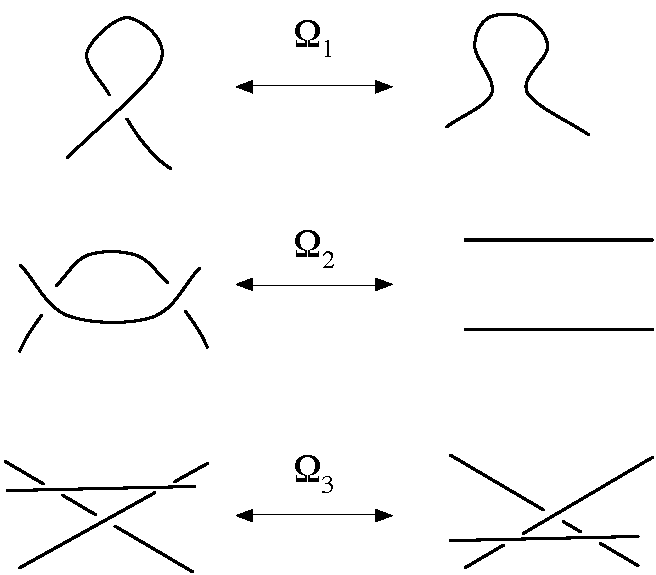
\includegraphics[width=3in]{Reidemeister123.pdf}
\caption{The three Reidemeister moves}
\label{RMoves}
\end{figure}

We first establish a lemma to our purposes, that shows we can clean up our knot diagram in a particularly suitable way.

Given a knot $K$ and a diagram $D(K)$ of $K$, we  call the application of a 
Reidemeister move $\rho$ a {\em neatening} move if the resulting diagram $D'(K)$ has a crossing number less than or
equal to the crossing number of $K$ i.e. any neatening move
of the type $\Omega_{1}$ or $\Omega_{2}$ can occur in
only one direction. Let $\hat{\rho}=\rho_{1}\cdots\rho_{n}$ be a sequence of successive Reidemeister moves on the
diagram $D(K)$ (with $n=0$ being the identity move). We call $\hat{\rho}$ a {\em neatening isotopy} if either
$n=0$ or  each
$\rho_{i}$
is a neatening move. If, in addition, at least one of the $\rho_{i}$ is a move of  type $\Omega_{1}$ or $\Omega_{2}$, we
call $\hat{\rho}$ a {\em cleaning isotopy} of $D(K)$. If $\rho_{n}$ is  move of  type $\Omega_{1}$ or $\Omega_{2}$, we
call $\hat{\rho}$ a {\em concise}  cleaning isotopy of $D(K)$

For a given diagram $D(K)$, the collection of all its neatening isotopies can be given a partial ordering: given
neatening isotopies $\hat{\rho}=\rho_{1}\cdots\rho_{n}$ and $\hat{\sigma}=\sigma_{1}\cdots\sigma_{m}$, we put
$\hat{\rho}\le\hat{\sigma}$ when $n\le m$ and $\rho_{i}=\sigma_{i}$  for all $i\le n$. This partial order restricts to the
the subcollection  of concise cleaning isotopies.

\begin{lemma}\label{simplificationLemma} For any knot  $K$
and knot diagram $D(K)$, we may reduce
$D(K)$ via a neatening isotopy to a diagram
$D'(K)$  having the property that no neatening isotopy of $D'(K)$ is a cleaning isotopy of $D'(K)$ .
\end{lemma}
\begin{proof} If the collection of cleaning isotopies of $D(K)$ is an empty one, then $D(K)$ is the desired diagram.
So assume there is at least one cleaning isotopy of $D(K)$.

The collection of concise cleaning isotopies of
$D(K)$
forms a partially ordered set. Since each
concise cleaning
isotopy reduces the
number of crossings in the diagram by at least 1, each chain in the partially order set has length bounded by the
number of crossings in $D(K)$. Select any maximal element $\hat{\rho}$ of the partially ordered set. Let $D'(K)$ be
the diagram derived from $D(K)$ by applying $\hat{\rho}$. 
\end{proof}



The lemma allows us to assume w.l.o.g. we are working with minimal
crossing diagrams.

\subsection{The Dowker-Thistlethwaite code}

The Dowker-Thistlethwaite code (``DT'') of a knot $K$  is obtained as follows:


Choose a point on $K$ and begin traversing $K$ , counting each
crossing you pass through. If $K$ has $n$ crossings, then (since every
crossing is visited twice) the count ends at $2n$. Label each crossing
with the value of the counter when it is visited (each crossing is
labeled twice).  Finally, when labeling a crossing with an even
number, prepend with the label with a minus sign if traversing
``under" the crossing.  All crossings end up being labeled by a pair
of integers whose absolute values run, \emph{in toto}, from $1$ to
$2n$. It is easy to see that each crossing is labeled with one odd
integer and one even integer. For each odd integer $j$ between $1$ and
$2n-1$ inclusive, let $\textrm{pairedWith}(j)$ be the even integer
with which it is paired.  The DT code is the sequence $1,
\textrm{pairedWith}(1), 3, \textrm{pairedWith}(3), \ldots, 2n-1,
\textrm{pairedWith}(2n-1)$.

\section{The encoding}

The guiding intuition at work in the encoding is to think of a knot
diagram as representing the schematic of a signal flow. The crossings
represent gates or circuits. The arcs between the crossings represent
wires between the circuits. Thus, the whole encoding is really a
problem in how to represent this signal flow as a process. This
problem then decomposes into representing the crossing circuits and
wiring the circuits appropriately. As we will see in the sequel, the
crossing circuit of the $i$-th crossing of a knot, $K$, is a process,
$\meaningof{C(i)}_{\pi}(x_0,x_1,y_0,y_1,u)$, parameterized in $4+1$
ports corresponding to the in-coming and out-going arcs between each
crossing together with an additional port representing the
synchronizer for letting signals `cross over' in the gates. From this
perspective, the shape of the encoding may be expressed as follows.

\begin{eqnarray}
  \lefteqn{\meaningof{K}_{\pi} =} \nonumber \\
  & & (v_0 ... v_{4n-1})( \Pi_{i = 0}^{n-1} (\nu \; u)\meaningof{C(i)}_{\pi}(v_{4i},...,v_{4i+3},u) \nonumber \\
  & & \; \; \; \; \; \; \; \; \; \; \; \; \; \; \; \; \; \; | \Pi_{i = 0}^{n-1} W(v_{\omega(i,0)},v_{\omega(i,1)})|W(v_{\omega(i,2)},v_{\omega(i,3)}) )
\end{eqnarray}

where $n$ is the crossing number of $K$, and $\omega: n \times 4 \to
2n$, gives the index into the list of ports, $v_0 ... v_{4n-1}$ used
to wire the crossing circuits together in a manner consistent with the
chosen knot diagram of $K$.

\subsection{An example: the trefoil as a process}
Before giving a formal account of the encoding we begin with an
example, showing how to represent the trefoil knot as a process. The
natural starting point is the process encoding of a crossing
circuit. To arrive at this construction we begin by observing that the simplest form of a
wire-like process, $W(x_0,x_1)$, between two end-points, $x_0$ and $x_1$, is coded
as the process that receives a signal at either one of its end-points and sends it
out the other and then resumes being a wire.

\begin{equation}
  W(x_0,x_1) := x_0?(s).x_1!(s).W(x_0,x_1) + x_1?(s).x_0!(s).W(x_0,x_1)
\end{equation}

As we shall see, however, the encoding requires buffering. Taking the
choice to put the bufferiing in the wire complicates the definition of
the wire process, but not the intuitions: it is an infinite capacity
perfect \footnote{Where \emph{perfect} means meassages are delivered
 exactly once, in order} buffer.

[Ed. note: This fact actually leaves us with a design choice: put the
buffering in the wire or put the buffering in the crossing. The first
choice simplifies the crossing encoding. i am not convinced, however,
that this is the best decision. In some sense, the crossing is the
primary machinery and as such should be responsible for it's own
buffering.]

\begin{eqnarray}
  W(x,y) & = & (\nu \; n \; m)(Waiting(x,n,m) | Waiting(y,m,n))
\end{eqnarray}

\begin{eqnarray}
%  W(x_0,x_1) := x_0?(s).x_1!(s).W(x_0,x_1) + x_1?(s).x_0!(s).W(x_0,x_1) 
 \lefteqn{ Waiting(x,c,n) =} \nonumber \\
 & & x?(v).(\nu \; m)(Cell(n,v,m) | Waiting(x,c,m)) \nonumber \\
 & & + c?(w).c?(c).Ready(x,c,n,w) \\
 \lefteqn{ Ready(x,c,n,w) =} \nonumber \\
 & & x?(v).(\nu \; m)(Cell(n,v,m) | Ready(x,c,m,w)) \nonumber \\
 & & + x!(w).Waiting(x,c,n) 
\end{eqnarray}

\begin{eqnarray}
  Cell(c,v,n) & = & c!(v).c!(n).0
\end{eqnarray}

\begin{figure}[tbp]
\centering
\scalebox{0.30}[0.300]{\includegraphics*[viewport=0 0 810 750]{TrefoilMethodIllustrationNoText}}
\caption{ Trefoil as process }
\end{figure}

Next, we note that a crossing circuit will have somewhat more
structure than a pair of wires between $x_0$ and $y_1$ and $x_1$ and
$y_0$. In particular, it must somehow code what it means for a wire to
cross over or under. We interpret this as a synchronization. The wire
crossing over is allowed to transmit the signal without waiting while
the under-crossing wire must wait for an additional input on a
synchronization channel. To alert the under-crossing wire that it may
now proceed, the over-crossing wire must fire off an output. Thus, setting
$(\vec{a}) = (x_0,x_1,y_0,y_1,u)$ a crossing circuit is coded as the
following process.

\begin{eqnarray}
  C(\vec{a}) & := & x_1?(s).y_0!(s).(C(\vec{a})|u!) + y_0?(s).x_1!(s).(C(\vec{a})|u!) \nonumber \\
  & & + x_0?(s).u?.y_1!(s).(C(\vec{a})) + y_1?(s).u?.x_0!(s).(C(\vec{a})) 
\end{eqnarray}

Then the process encoding of the trefoil knot is essentially a
parallel composition of three crossing circuits. The main property we
must ensure is that the crossing circuits are connected to each other
in a way that respects the knot diagram. Additionally, we make each
synchronization channel local to each crossing via a restriction on
that channel.

\begin{eqnarray}
  \lefteqn{\meaningof{K_3}_{\pi} =} \nonumber \\
  & & (v_0 ... v_{5}) (\nu \; u_0)C(v_0,v_1,v_2,v_3,u_0) \nonumber \\
  & & \; \; \; \; \; \; \; \; \; \; \; \; | W(v_2,v_7) | W(v_3,v_6) \nonumber \\
  & & \; \; \; \; \; \; \; \; \; \; \; \; | (\nu \; u_1)C(v_4,v_5,v_6,v_7,u_1) \nonumber \\
  & & \; \; \; \; \; \; \; \; \; \; \; \; | W(v_4,v_9) | W(v_5,v_8) \nonumber \\
  & & \; \; \; \; \; \; \; \; \; \; \; \; | (\nu \; u_2)C(v_8,v_9,v_{10},v_{11},u_2) \nonumber \\
  & & \; \; \; \; \; \; \; \; \; \; \; \; | W(v_{10},v_0) | W(v_{11},v_1)
\end{eqnarray}

\subsection{The general encoding}

As we have already seen in the example how to code up a crossing
circuit, the only thing that remains is to show how to wire the
crossing circuits together in a manner consistent with a knot
diagram. To do this we make use of the DT code. We recognize that the
(lexicographically least) DT code is only unique for prime knots. This
is not really a limitation of our approach as we will demonstrate in a
subsequent section.

\begin{itemize}
   \item From a DT code, $DT(K)$, of a knot $K$ we recover a parity
     reversing involution $p: 2n \to 2n$, where $n$ is the crossing
     number of $K$, as well as an ordering on the crossings.
   \item Observe that the process encoding of the knot will consume
     exactly $2n$ ports for wiring up the $x0,...,y1$ positions of the
     crossing circuits.
   \item Let $C(i)$ denote the $i$-th crossing of $K$ in the ordering
     implied by the DT code, $DT(K)$. The constraints in the figure
     below (DT-constraints) uniquely determine a wiring of the
     crossing circuits, expressed in the map $\omega: n \times 4 \to
     2n$, that respects the connections of the crossings.
     \begin{figure}[tbp]
        \begin{eqnarray}
          y_0(C(i)) & = & x_0(C(i-1)) \nonumber \\
          y_1(C(i)) & = & x_1(C(p(i)-1)) \nonumber \\
          x_0(C(i)) & = & y_0(C(i+1)) \nonumber \\
          x_1(C(i)) & = & y_1(C(p(i)+1)) \nonumber
        \end{eqnarray}
%        \begin{tabular}{cccc}
%          $y_0(C(i)) = x_0(C(i-1))$ & $\; y_1(C(i)) = x_1(C(p(i)-1))$ & $\; x_0(C(i)) = y_0(C(i+1)) \;$ & $\; x_1(C(i)) = y_1(C(p(i)+1))$ \\
%        \end{tabular}
       \caption{DT-constraints}
   \end{figure}
    where we use $s_i(C(i))$ to denote the port used in the $s_i$
    position of the encoding of the $i$th crossing and all arithmetic is
    mod $2n$. 
 \end{itemize}

 This result may be derived from a small tweak to Scharein's
 derivation of the graph sometimes called the knot shadow from a DT
 code \cite{SchareinPhD}.  

\begin{remark}
  We observe that it is possible to compress considerably the
  expression of these constraints. Let $s$ range over $\{x,y\}$, and
  define the involution $\hat{(-)}: \{x,y\} \to \{x,y\}$ by $\hat{x} =
  y$, $\hat{y} = x$, and let $\chi : \{x,y\} \to \{0,1\}$ be defined by
  $\chi(x) = 1$, $\chi(y) = 0$. Our constraints may be expressed by the
  single equation

  \begin{equation}
    s_i(C(i)) = \hat{s_i}(C(p^i(i) + (-1)^{\chi(s)+1}))
  \end{equation}
  
  The advantage of expressing the constraints in this more compressed
  way is that the two `switching conditions' are more prominently
  evident. Firstly, $x$ positions are always wired to $y$
  positions. Secondly, left-hand-side ports are always wired to
  predecessor (respectively sucessor) crossings using the index, while
  right-hand-side ports are always wired to predecessor (respectively
  successor) crossings using $p$ of the index.

  More generally, the encoding respects the discipline that both
  inter- and intra-crossing wires are always $x$ to $y$ while
  inter-crossing wires take $\__i$ positions to $\__i$ positions and
  intra-crossing wires take $\__i$ positions to $\__{i+1}$
  positions. In some very real sense, this discipline is the essence
  of what it means to cross.
\end{remark}

\section{Ambient isotopy as weak bisimilarity} \label{MainThm}

\begin{theorem}[main]
  Two knots, $K_0$ and $K_1$ are ambient isotopic, written here $K_0
  \sim K_1$, iff their encodings as processes are weakly bisimilar,
  i.e.
  \begin{equation}
    K_0 \sim K_1 \iff \meaningof{K_0}_{\pi} \simeq \meaningof{K_1}_{\pi}
  \end{equation}
\end{theorem}

\subsection{One direction}

In this section we show that if two knots are ambient isotopic then
their encodings as processes are bisimilar. Since two knot(
presentation)s are ambient isotopic if and only if there is a sequence
of Reidemeister moves transforming one presentation to the other
(\cite{sossinskyknotsandbraids}), it suffices to show that the
encodings of the Reidemeister moves as operations on processes
preserve bisimilarity.

\begin{lemma}[Reidemeister preserves bisimilarity] For each Reidemeister move, $\Omega_i$ if $K
  \stackrel{\Omega_i}{\longrightarrow} K'$ then $\meaningof{K}_{\pi} \simeq \meaningof{K'}_{\pi}$.
\end{lemma}

\subsubsection{Encoding the Reidemeister moves}

The proof method simply encodes the left hand and right hand side of
the Reidemeister moves. In each case it is easy to see that
corresponding processes are bisimilar. See \ref{encodingRMoves}

\begin{equation}
  \meaningof{L(\Omega_i)}_{\pi}(\vec{x}) \simeq \meaningof{R(\Omega_i)}_{\pi}(\vec{x})
\end{equation}

\begin{remark}
  Up to this point, when referring to the encoding of a knot as a
  process, we have been ignoring the fact that a given knot may have
  many diagrams. Because the Reidemeister moves (as operations on
  processes) preserve bisimilarity this ignorance can remain a blissful
  state.
\end{remark}

\subsection{The other direction}

The intuitive argument runs as follows. Suppose $K_0, K_1$ such that
$\meaningof{K_0}_{\pi} \sim \meaningof{K_1}_{\pi}$. For any crossing
$C_i(x_{0},x_{1},y_{0},y_{1},u)$ of $\meaningof{K_{i \bmod 2}}_{\pi}$
there are exactly four transitions possible. W.l.o.g. we may consider
only two of them: one for the over-crossing and one for the
under-crossing. Of the two, only one of them (the over-crossing
transition) immediately enables a transition in another
crossing. Because of the DT-constraints we know that only one such
crossing is so enabled, and only one of its transition is enabled. We
think of this as the `successor' crossing of the current one. Note
that the DT-constraints do not determine whether the over- or
under-crossing is enabled, but \emph{eventually} (i.e. in the presence
of at least two signals or pulses to the knot-process) the successor
crossing enables its successor. The DT-constraints ensure that we may
continue in this way visiting every crossing exactly twice.

Because $\meaningof{K_{i}}_{\pi} \sim \meaningof{K_{i+1 \bmod
    2}}_{\pi}$, $\meaningof{K_{i+1 \bmod 2}}_{\pi}$ must mimick the
path we have traced. Further, bisimulation is symmetric and so our
argument may be run from $\meaningof{K_{i+1 \bmod 2}}_{\pi}$ to
$\meaningof{K_{i}}_{\pi}$. Thus, the bisimulation establishes a
bijection between the crossings of $K_{0}$ and $K_{1}$ that preserves
the polarity (i.e. over/under relationships) and the connections
between the crossings. Thus, $K_{0}$ is in the same ambient isotopy
class as $K_{1}$.

\section{Discussion}

\subsection{From prime knots to composites via parallel composition}

We can compose knots in the process representation by rewiring
crossings in a manner that respects the DT-constraints. Taking
advantage of the compositional nature of the encoding, and recalling
equation \ref{linkingident} in \ref{linkingabs} we see that

\begin{eqnarray}
  \meaningof{K}_{\pi} & \equiv & (\meaningof{K}_{\pi} - \meaningof{C(j)}_{\pi}) \# \meaningof{C(j)}_{\pi}
\end{eqnarray}

(eliding the restriction scope on $\meaningof{C(j)}_{\pi}$ and its arguments).

Similarly, we can provide a more compact notation for wiring two crossing circuits together.

\begin{eqnarray}
  & \meaningof{C_0(k)}_{\pi} \smallsmile \meaningof{C_1(k')}_{\pi} & \nonumber \\
  & \triangleq & \nonumber \\
  & ( w_0 w_1)\meaningof{C_0(k)}_{\pi}(v_{\omega(k,0)},v_{\omega(k,1)},w_0,w_1,u_i) & \nonumber \\
  & | \meaningof{C_1(k')}_{\pi}(w_0,w_1,x_{\omega(k',2)},x_{\omega(k',3)},u_j) &
\end{eqnarray}

allowing us to write

\begin{eqnarray}
  & \meaningof{K_0 + K_1}_{\pi} & \nonumber \\
  & = & \nonumber \\
  & (\meaningof{K_0}_{\pi} - \meaningof{C_0(k)}_{\pi}) \# (\meaningof{C_0(k)}_{\pi} \smallsmile \meaningof{C_1(k')}_{\pi}) \# (\meaningof{K_1}_{\pi} - \meaningof{C_1(k')}_{\pi}) &
\end{eqnarray}

This construction not only illustrates, as previously promised, that
the method of encoding is not restricted to prime knots, but that
there is a good conceptual fit between the domain and the
representation: the notion of composition of knots lines up with a
form of parallel composition of processes. It should be
mentioned in this connection that there is nothing in the proof of the
main theorem that in any way depends on primality of the knots being
compared.

\subsection{Old invariants from new: the Kauffman bracket}

We also observe that the representation is particularly natural for
working with skein relations as in the Kauffman bracket. In
particular, we may recursively define a function, $\langle\!\langle - \rangle\!\rangle$, taking a
process, $P$ in the image of our encoding of knots to a Laurent
polynomial (the Kauffman bracket of the knot $P$ encodes).

To make the encoding more intuitive and well-aligned with the standard
definition it will be useful to add a few more items to our toolbox. First, we have the following
operators on crossing circuits

\begin{eqnarray}
  C^{\asymp}(j) & \triangleq & W(v_{\omega(j,0)},v_{\omega(j,1)}) | W(v_{\omega(j,2)},v_{\omega(j,3)}) \nonumber \\
  C^{)(}(j) & \triangleq & W(v_{\omega(j,0)},v_{\omega(j,2)}) | W(v_{\omega(j,1)},v_{\omega(j,3)})
\end{eqnarray}

representing the two ways to wire the ports of the crossing circuit to avoid the crossing.

Next, we characterize a \emph{cycle}, which will represent for us the
class of processes corresponding to the unknot, as any process $R$,
structurally equivalent to a process of the form $\Pi_{i = 0}^{k-1}
W(v_i,v_{i+1 \bmod k})$, for some $k$.

Then our function, $\langle\!\langle - \rangle\!\rangle$, is determined by the constraints

\begin{enumerate}
  \item \begin{eqnarray}
      \langle\!\langle(K-j) \# C(j)\rangle\!\rangle & = & a \langle\!\langle(K-j) \# C^{\asymp}(j)\rangle\!\rangle  + a^{-1} \langle\!\langle(K-j) \# C^{)(}(j)\rangle\!\rangle
    \end{eqnarray}

  \item for any cycle, $R$, that 
    \begin{equation}
      \langle\!\langle( v_0 ... v_{2n-1})R\rangle\!\rangle = 1
    \end{equation}

  \item \begin{eqnarray}
      \langle\!\langle( v_0 ... v_{2n-1})(P | R)\rangle\!\rangle & = & (-a^2 - a^{-2})\langle\!\langle( v_0 ... v_{2n-1})P\rangle\!\rangle
    \end{eqnarray}
  \end{enumerate}

  corresponding to the usual equations defining the Kauffman bracket:

\begin{enumerate}
\item $\bigl<
   \xygraph{              % The crossing
     !{0;/r1.0pc/:}
     [u(0.5)]
     !{\xunderv}
   }
 \bigr> 
 =
 a\bigl<\hspace{0.1pc} % The horizontal crossing eliminated
   \xygraph{
     !{0;/r1.0pc/:}
     [u(0.5)]
     !{\xunoverv}
   }\hspace{0.1pc}
 \bigr> 
 +
 a^{-1}\bigl<\hspace{0.1pc} % the vertical crossing eliminated
 \xygraph{
  !{0;/r1.0pc/:}
       [u(0.5)]
  !{\xunoverh}
}\hspace{0.1pc}
\bigr>
 $

 \item $ \bigl<\hspace{0.1pc} 
 \xygraph{                          % the unknot
 !{0;/r1.0pc/:}
 !{\vcap-}
 !{\vcap+}
 }
 \hspace{0.1pc}
 \bigr>
 =1
 $
 
 \item $
 \bigl<\hspace{0.1pc}
 L \bigsqcup 
  \xygraph{               % the unknot, again
 !{0;/r1.0pc/:}
 !{\vcap-}
 !{\vcap+}
 }
 \hspace{0.1pc}\bigr>
 =
 (-a^{2}-a^{-2})\bigr<\hspace{0.1pc}L\hspace{0.1pc}\bigr>$
\end{enumerate}

\section{Conclusions and future work}

\paragraph{Braids, tangles and virtual knots}

As may be seen from the encoding of the Reidemeister moves, nothing in
this approach restricts it to knots. In particular, the same
techniques may be lifted to braids and tangles. More generally,
Kauffman posits an intriguing new member to the knot family by
virtualizing the crossings in a knot diagram
\cite{kauffman-2005-VKNL}. We note that while we arrived at this
encoding before becoming aware of Kauffman's work, this line of
investigation is very much in line with the intuitions guiding the
encoding presented here. Specifically, we see no reason why the
crossing circuit cannot be any $\pi$-calculus process that respects
the interface of crossing circuit presented here.

\paragraph{Other calculi, other bisimulations and geometry as behavior}

Of course, the astute reader may have noticed that the encoding
described here is not much more than a linear notation for a minimal
graph-based representation of a knot diagram. In this sense, there is
nothing particularly remarkable about the representation. Though
expressed in a seemingly idiosyncratic way, it's more or less the same
information that any freely downloadable program for calculating knot
polynomials uses routinely. What is remarkable about this
representational framework is that it enjoys an \emph{independent}
interpretation as the description of the behavior of concurrently
executing processes. Moreover, the notion of the equivalence of the
behavior of two processes (in the image of the encoding) coincides
exactly with the notion of ambient isotopy. It is the precise
alignment of independently discovered notions that often indicates a
phenomena worth investigating.

This line of thought seems particularly strengthened when we recall,
as we did in the introduction, the $\pi$-calculus is just one of many
`computational calculi' that may be thought of as an
\emph{algebra+computational dynamics} and that virtually every such calculus
is susceptible to a wide range of bisimulation and bisimulation up-to
techniques. As such, we see the invariant discussed here as one of
many potential such invariants drawn from these relatively new
algebraic structures. It is in this sense that we see it as a new kind
of invariant and is the inspiration for the other half of the title of
this paper.

Finally, if the reader will permit a brief moment of philosophical
reflection, we will conclude by observing that such a connection fits
into a wider historical context. There is a long-standing enquiry and
debate into the nature of physical space. Using the now familiar
signposts, Newton's physics -- which sees space as an absolute
framework -- and Einstein's -- which sees it as arising from and
shaping interaction -- we see this connection as fitting squarely
within the Einsteinian weltenschauung. On the other hand, we cannot
help but notice that unlike the particular mathematical framework in
which Einstein worked out his programme -- a framework that required
continuity -- behavior and the implied notions of space and time are
entirely discrete in this setting, built out of names and acts of
communication. In this light we look forward to revisiting the now
well-established connection between the various knot invariants such
as the Kauffman bracket and quantum groups. Specifically, it appears
that the kinematic picture of loop quantum gravity derived from spin
networks can be faithfully encoded in a manner analogous to one used
here to encode knots, but the process structure offers an account of
dynamics somewhat different from spin foams \cite{baez-2000-543}.


\paragraph{Acknowledgments.}
The author wishes to acknowledge his longstanding debt to Samson
Abramksy for making so accessible his foundational insights into the
Curry-Howard isomorphism.

% ------------------------------------------------------------------------
%GATHER{Xbib.bib}   % For Gather Purpose Only
%GATHER{Paper.bbl}  % For Gather Purpose Only
\bibliographystyle{plain}
\bibliography{icalp}

% ------------------------------------------------------------------------

% ------------------------------------------------------------------------

\section{Appendix: linking abstractions and other process constructions} \label{linkingabs}

In the sequel we will find it useful to adapt some of Milner's
additional process constructions, such as the one for linking
abstractions. Given abstractions $F = (\vec{x})P$, and $G =
(\vec{y})Q$ with $|F|, |G| \geq j$ we may compose them, gluing
channels $x_{|F|-{j+1}},...,x_{|F|-1}$ to channels
$y_{0},...,y_{i'+j}$ by

\begin{eqnarray}
  & F \#_j G & \nonumber \\
  & \triangleq & \nonumber \\
  & (z_0,...,z_{|F|+|G|-(j+1)})(F\langle z_0,...,z_{|F|-1} \rangle | G\langle z_{|F|-{j+1}},..., z_{|F|+|G|-(j+1)}\rangle) &
\end{eqnarray}

We may omit the subscript, $_j$, when it is clear from context. Note
that the operation is associative, allowing us to write $F\#G\#H$
unambiguously.

Additionally, for an abstraction of the form, $F =
(\vec{z})\Pi_{i=0}^kP_i\langle z_{f(i,0)},...,z_{f(i,n_i)} \rangle$ with
$f$ and indexing function into the formals, $\vec{z}$, of the
abstraction, we write

\begin{eqnarray}
  F - P_j \triangleq (\vec{v})\Pi_{i=0}^{j-1}P_i\langle v_{f(i,0)},...,v_{f(i,n_i)}\rangle|(\vec{v})\Pi_{i=j+1}^{k}P_i\langle v_{f(i,0)},...,v_{f(i,n_i)} \rangle
\end{eqnarray}

to denote the deletion of the process $P_j$ from the parallel
composition. Thus, we have

\begin{eqnarray} \label{linkingident}
  F \equiv (F - P_j)\#P_j
\end{eqnarray}

\section{Appendix: encoding the Reidemeister moves}\label{encodingRMoves}

To facilitate the encoding we define a short-circuit process. Its
primary difference in behavior from a wire is that it is also willing
to offer a communication on the synchronizer channel associated with a
crossing circuit, and when composed with a crossing circuit makes a
wire.

\begin{eqnarray}
  S(x_0,x_1,u) & := & x_0?(s).x_1!(s).S(x_0,x_1,u) + x_1?(s).x_0!(s).S(x_0,x_1,u) \nonumber \\
  & & + u!.S(x_0,x_1,u)
\end{eqnarray}

\paragraph{$\Omega_1$}

\begin{eqnarray}
  \meaningof{L(\Omega_1)}_{\pi}(x_0,x_1) & := & (\nu \; z_0 z_1 u_0)(S(z_0,z_1,u_0) | C(z_0,z_1,x_0,x_1,u_0)) \\
  \meaningof{R(\Omega_1)}_{\pi}(x_0,x_1) & := & W(x_0,x_1)
\end{eqnarray}

\paragraph{$\Omega_2$}

\begin{eqnarray}
  \meaningof{L(\Omega_2)}_{\pi}(x_0,x_1,y_0,y_1) & := & (\nu \; z_0 z_1 u_0)(C(x_0,x_1,z_0,z_1,u_0) \nonumber \\
  & & | C(z_0,z_1,y_0,y_1,u_0)) \\
  \meaningof{R(\Omega_2)}_{\pi}(x_0,x_1,y_0,y_1) & := & W(x_0,y_0) | W(x_1,y_1)
\end{eqnarray}

\paragraph{$\Omega_3$}

\begin{eqnarray}
  \meaningof{L(\Omega_3)}_{\pi}(x_0,x_1,y_0,y_1,w_0,z_0) & := & (\nu \; u_0 v_0 w_1 z_1)(C(x_0,x_1,v_0,z_1,u_0) \nonumber \\
  & & | C(w_0,v_0,z_0,w_1,u_0) \nonumber \\
  & & | C(w_1,z_1,y_0,y_1,u_0)) \\
  \meaningof{R(\Omega_3)}_{\pi}(x_0,x_1,y_0,y_1,w_0,z_0) & := & (\nu \; u_0 v_0 w_1 z_1)(C(x_0,x_1,v_0,z_1,u_0) \nonumber \\
  & & | C(v_0,w_1,y_0,y_1,u_0) \nonumber \\
  & & | C(z_1,w_0,w_1,z_0,u_0)) \\
\end{eqnarray}

\end{document}
% ------------------------------------------------------------------------
